% Chapter Template

\chapter{Conclusions and Future Work} % Main chapter title

\label{Chapter5} % Change X to a consecutive number; for referencing this chapter elsewhere, use \ref{ChapterX}

%----------------------------------------------------------------------------------------
%	SECTION 1   % TARGET 1500 WORDS IN THIS CHAPTER
%----------------------------------------------------------------------------------------

\section{Overview}
This chapter provides concluding remarks on the deliverables of the previous chapter and provides a discussion on aspects where the project would benefit moving foward.

%----------------------------------------------------------------------------------------
%	SECTION 2
%----------------------------------------------------------------------------------------

\section{MEGAphone Chassis/Case First Revision}
The MEGAphone accessible chassis project was fully realised on the 8th of November, 2020. 
In this chapter, the development of the project and how various aspects benefit the usability of the MEGAphone device as a whole, will be analysed. % maybe add to overview
Additionally, a discussion on the potential future work of the project will estabilish how to best approach a succeeding revision of the chassis and the MEGAphone PCB followed by some concluding remarks. \newline

This thesis has answered the following research questions in the preceding chapters:
\begin{enumerate}
    \item What is the relationship between Digital Sovereignty and Universal Design?
        \begin{enumerate}
        \item[-] ...
        \end{enumerate} 
    \item Why is Universal Design important in the design of products today?
        \begin{enumerate}
        \item[-] ...
        \end{enumerate}
    \item Why is Digital Sovereignty important in the design of electronic products today?
        \begin{enumerate}
        \item[-] ...
        \end{enumerate} 
    \item How can the seven design principles be used in the design of the MEGAphone case to support those with disabilities?
        \begin{enumerate}
        \item[-] ...
        \end{enumerate} 
    \item How can the 'Right to Repair' mantra be used in support of the universally designed MEGAphone case?
        \begin{enumerate}
        \item[-] ...
        \end{enumerate} 
    \item What are the effects of COVID-19 on Digital Sovereignty, Universal Design and the MEGAphone project?
        \begin{enumerate}
        \item[-] ...
        \item[-] ...
        \end{enumerate} 
\end{enumerate}

% %-----------------------------------
% %	SUBSECTION 1
% %-----------------------------------
\subsection{Subsection 1}
//

% %-----------------------------------
% %	SUBSECTION 2
% %-----------------------------------
\subsection{Subsection 2}
//


%----------------------------------------------------------------------------------------
%	SECTION 3
%----------------------------------------------------------------------------------------
\section{Future Work}
The following section addresses both the MEGAphone PCBs and the accessible chassis and discusses the recommendations in regard to the project moving forward.

%-----------------------------------
%	SUBSECTION 1
%-----------------------------------
\subsection{Original PCB Layout}
% analyse the changes in the final design, what limitations the existing PCB layout has and propose a better layout that satisfies the UD principles, talk about what is ideal and what is the best that can be done with current layout. 
% Ideal layout includes ports at top of device along with rocker switches replacing current rev2 switches on the main PCB

The layout of the second revision MEGAphone PCB served as the major constraint of this project, as the case design had to be designed around it without any significant redesign due to the complexity of the device. 
Certain reworks to better adapt the design to an accessible interface included removing the existing switches in favour of larger rocker switches hosted on an external PCB (view figure).

\begin{figure} [h]
\begin{centering}
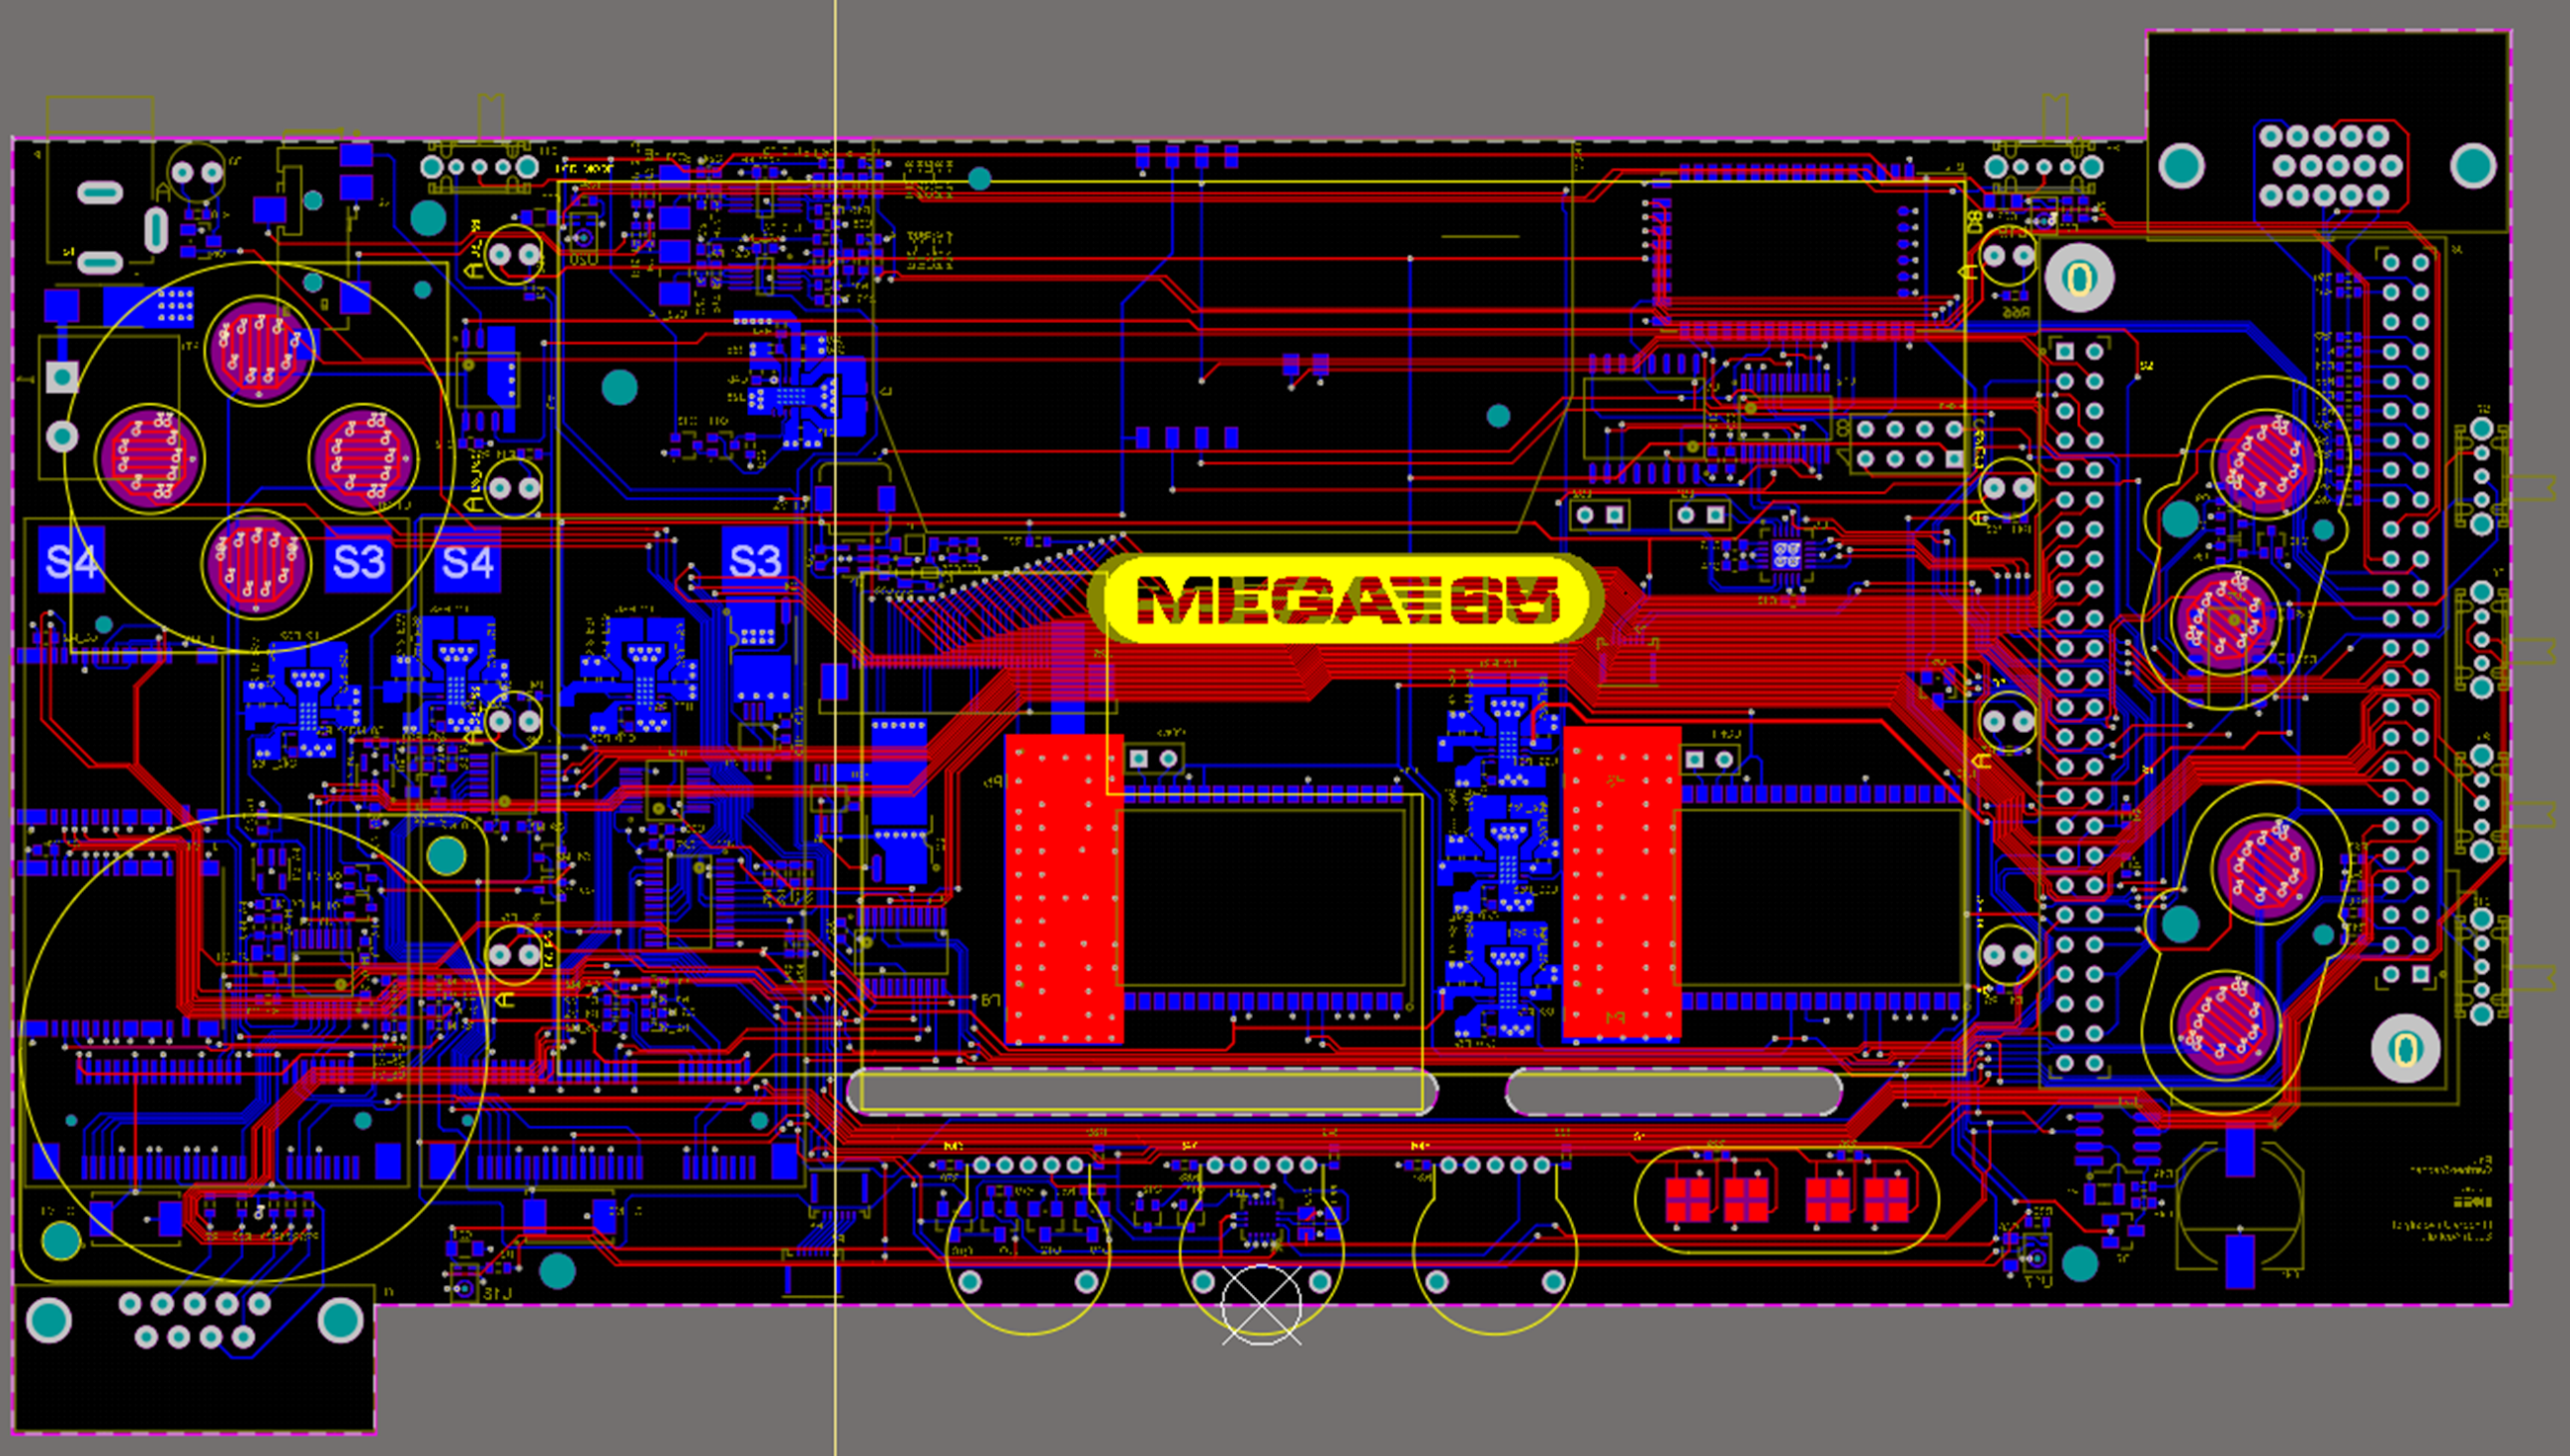
\includegraphics[width=10cm,height=10cm,keepaspectratio]{Figures/pcb_original.png}
\caption{This is the PCB layout as it was during the course of development of this project.}
\label{fig:ThisFig}
\end{centering}
\end{figure}

%-----------------------------------
%	SUBSECTION 2
%-----------------------------------
\subsection{Proposed PCB Layout}

A possible solution to the existing PCB which does inhabit the Universal Design principles is proposed in FIGURE. 
The underlying idea with this redesign was to integrate the design all onto one PCB. 
Doing so would reduce the amount of wires required and given that those in the current solution are soldered to make space, it makes the design overall ‘simpler’.

\begin{figure} [h]
\begin{centering}
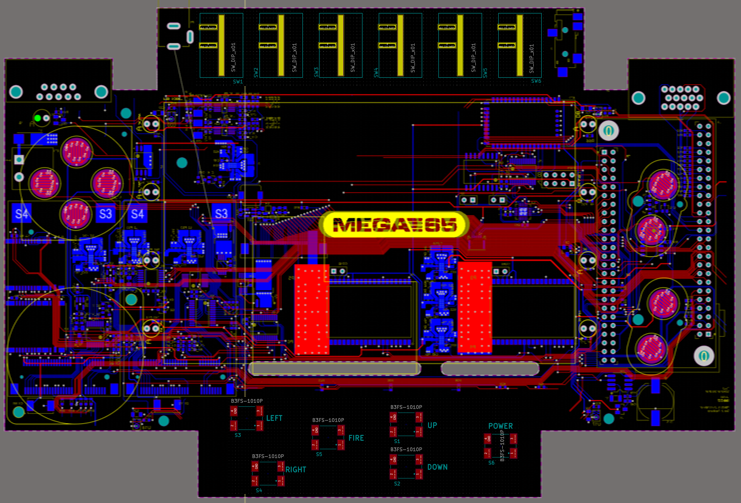
\includegraphics[width=10cm,height=10cm,keepaspectratio]{Figures/pcb_final.png}
\caption{This is the PCB as it is proposed in a future revision of the MEGAphone project.}
\label{fig:ThisFig}
\end{centering}
\end{figure}

In order to make the device more intuitive, placement of the 9-pin DSUB port should be moved to the ‘top’ of the device in the same orientation as the VGA port, so that users know from a glance that this is where all device ports are expected to be.
The accessible button interface also utilises an external PCB which hosts the tactile switches that were opted to form the base of the accessible button function. 
Other options were considered, such as silicone rubber pads, as used for the directional button and ‘A’, ‘B’ buttons. 
However, primarily due to the size, larger buttons would be recommended as this would make button presses easier for all users, disregarding the EZ keys in this scenario.

It is also recommended that the device incorporates multiple 3.5mm jack inputs, separate from the audio function, in its design as this can give users the ability to plug in multiple switches much like the Jellybean presented in this project.
Microsoft's accessible controller \cite{adaptive} is a prime example of the usefulness of this feature and for those who might not be able to interact with the EZ keys or Gameboy buttons but desire their own means of interaction with the device, multiple inputs allows for multiple unique functions.

%----------------------------------------------------------------------------------------
%	SECTION 4
%----------------------------------------------------------------------------------------

\section{Final Summary}
//